\documentclass[english,floatsintext,man]{apa6}

\usepackage{amssymb,amsmath}
\usepackage{ifxetex,ifluatex}
\usepackage{fixltx2e} % provides \textsubscript
\ifnum 0\ifxetex 1\fi\ifluatex 1\fi=0 % if pdftex
  \usepackage[T1]{fontenc}
  \usepackage[utf8]{inputenc}
\else % if luatex or xelatex
  \ifxetex
    \usepackage{mathspec}
    \usepackage{xltxtra,xunicode}
  \else
    \usepackage{fontspec}
  \fi
  \defaultfontfeatures{Mapping=tex-text,Scale=MatchLowercase}
  \newcommand{\euro}{€}
\fi
% use upquote if available, for straight quotes in verbatim environments
\IfFileExists{upquote.sty}{\usepackage{upquote}}{}
% use microtype if available
\IfFileExists{microtype.sty}{\usepackage{microtype}}{}

% Table formatting
\usepackage{longtable,booktabs}
\usepackage[counterclockwise]{rotating}   % Landscape page setup for large tables
\usepackage{multirow}		% Table styling
\usepackage{tabularx}		% Control Column width
\usepackage[flushleft]{threeparttable}	% Allows for three part tables with a specified notes section
\usepackage{threeparttablex}            % Lets threeparttable work with longtable
\usepackage{longtable}              % Allows tables to break across pages

  \usepackage{graphicx}
  \makeatletter
  \def\maxwidth{\ifdim\Gin@nat@width>\linewidth\linewidth\else\Gin@nat@width\fi}
  \def\maxheight{\ifdim\Gin@nat@height>\textheight\textheight\else\Gin@nat@height\fi}
  \makeatother
  % Scale images if necessary, so that they will not overflow the page
  % margins by default, and it is still possible to overwrite the defaults
  % using explicit options in \includegraphics[width, height, ...]{}
  \setkeys{Gin}{width=\maxwidth,height=\maxheight,keepaspectratio}
\ifxetex
  \usepackage[setpagesize=false, % page size defined by xetex
              unicode=false, % unicode breaks when used with xetex
              xetex]{hyperref}
\else
  \usepackage[unicode=true]{hyperref}
\fi
\hypersetup{breaklinks=true,
            pdfauthor={},
            pdftitle={How to do Effective and Successful Bank Telemarketing},
            colorlinks=true,
            citecolor=blue,
            urlcolor=blue,
            linkcolor=black,
            pdfborder={0 0 0}}
\urlstyle{same}  % don't use monospace font for urls

\setlength{\parindent}{0pt}
%\setlength{\parskip}{0pt plus 0pt minus 0pt}

\setlength{\emergencystretch}{3em}  % prevent overfull lines

\setcounter{secnumdepth}{0}
\ifxetex
  \usepackage{polyglossia}
  \setmainlanguage{}
\else
  \usepackage[english]{babel}
\fi

% Manuscript styling
\captionsetup{font=singlespacing,justification=justified}
\usepackage{csquotes}

 % Line numbering
  \usepackage{lineno}
  \linenumbers


\usepackage{tikz} % Variable definition to generate author note

% fix for \tightlist problem in pandoc 1.14
\providecommand{\tightlist}{%
  \setlength{\itemsep}{0pt}\setlength{\parskip}{0pt}}

% Essential manuscript parts
  \title{How to do Effective and Successful Bank Telemarketing}

  \shorttitle{Predictive Modeling with Logistic Regression}


  \author{
          Arindam Barman\textsuperscript{1},
          Mohamed Elmoudni\textsuperscript{1},
          Shazia Khan\textsuperscript{1},
          Kishore Prasad\textsuperscript{1}  }

  \def\affdep{{"", "", "", ""}}%
  \def\affcity{{"", "", "", ""}}%

  \affiliation{
    \vspace{0.5cm}
          \textsuperscript{1} City University of New York (CUNY)  }


%   \def\affinst{{"init", "City University of New York (CUNY)"}}%
%   \def\affstate{{"init", ""}}%
%   \def\affcntry{{"init", ""}}%

 % If no note is defined give only author information if available
    \note{
    \vspace{1cm}
    Author note

    \raggedright
    \setlength{\parindent}{0.4in}

    \newcounter{author}

%     %       %       \setcounter{author}{0}
%         %           \addtocounter{author}{1}
%         %         \expandafter\edef\csname authorid\endcsname{\theauthor}
%         Arindam Barman, \pgfmathparse{\affdep[\authorid]} \pgfmathresult, \pgfmathparse{\affinst[\authorid]} \pgfmathresult, \pgfmathparse{\affcity[\authorid]} \pgfmathresult, \pgfmathparse{\affstate[\authorid]} \pgfmathresult, \pgfmathparse{\affcntry[\authorid]} \pgfmathresult
%       %     ;
%     %       %       \setcounter{author}{0}
%         %           \addtocounter{author}{1}
%         %         \expandafter\edef\csname authorid\endcsname{\theauthor}
%         Mohamed Elmoudni, \pgfmathparse{\affdep[\authorid]} \pgfmathresult, \pgfmathparse{\affinst[\authorid]} \pgfmathresult, \pgfmathparse{\affcity[\authorid]} \pgfmathresult, \pgfmathparse{\affstate[\authorid]} \pgfmathresult, \pgfmathparse{\affcntry[\authorid]} \pgfmathresult
%       %     ;
%     %       %       \setcounter{author}{0}
%         %           \addtocounter{author}{1}
%         %         \expandafter\edef\csname authorid\endcsname{\theauthor}
%         Shazia Khan, \pgfmathparse{\affdep[\authorid]} \pgfmathresult, \pgfmathparse{\affinst[\authorid]} \pgfmathresult, \pgfmathparse{\affcity[\authorid]} \pgfmathresult, \pgfmathparse{\affstate[\authorid]} \pgfmathresult, \pgfmathparse{\affcntry[\authorid]} \pgfmathresult
%       %     ;
%     %       %       \setcounter{author}{0}
%         %           \addtocounter{author}{1}
%         %         \expandafter\edef\csname authorid\endcsname{\theauthor}
%         Kishore Prasad, \pgfmathparse{\affdep[\authorid]} \pgfmathresult, \pgfmathparse{\affinst[\authorid]} \pgfmathresult, \pgfmathparse{\affcity[\authorid]} \pgfmathresult, \pgfmathparse{\affstate[\authorid]} \pgfmathresult, \pgfmathparse{\affcntry[\authorid]} \pgfmathresult
%       %     .

                                                      }
  
  

\begin{document}

\maketitle



\section{Abstract}\label{abstract}

The objective of this project is to analyze and improve a Portuguese
bank's telemarketing campaign efficiency by identifying socio-economic
attributes of customers as the driving factor for term deposit product
selection. As methodology, we will be using the Cross Industry Data
Standard Process for Data Mining (CRISP DM) framework for this project.
We will start with the business case, followed by data exploration, data
preparation, modeling, evaluation, and recommendation from final model.
The dataset has 16 variables related to customer's socio-economic
conditions and about 41188 customer records. The response is binary
variable, the campaign response. We will create different models -
Logistic Regression, Classification Tree, and Random Forest. To evaluate
and select from the three models, we used accuracy, (AUC), F1 score etc.
With the given dataset, the response is disproportionate to the
population with 10\% success. This specific correlation incurred some
challenges in the model. Hence we had to use the Area under curve (AUC)
metrics for our final selection rather than the accuracy number. Based
on our model comparison Random Forest has been found as the most
efficient model with AUC score of around 92\% for the given case
scenario. Among predictor variables, we found that the
\enquote{duration} variable is the most important predictor; with longer
duration calls resulting into more productive discussions and success of
the campaign. The next important predictor variables are inter-bank
transfer rate (euribor3m) and (nr.employed), high transfer rates and
number of bank employees respectively lead to successful campaigns.

\section{Keywords}\label{keywords}

\enquote{Logistics Regression Model, Classification Tree, Random Forest,
Area under curve (AUC), Predictive modeling, Bank Telemarketing, Direct
Marketing, Data Mining}

\section{Introduction}\label{introduction}

Banks are increasingly concerned about their investment in marketing
campaigns. High and fierce bank competitions have reduced the response
rate from marketing campaigns to low, sometimes close to single digit.
Consequently, banks have invested aggressively in their marketing
campaigns to overcome competition and gain edge over their competitors.
Adversely, negative impact of mass campaigns also influences bank's
brand and value.

Banking companies have started working on addressing this tradeoff. One
solution is to be able to identify customers who may have higher chances
of response to a marketing campaign. Although the solution is intuitive,
it carries multiple challenges such as methods on how to identify those
customers and target them for higher responses, the accuracy of
predicting responses, and maintaining response success rate above
expectations.

Therefore, our objective in this project is to develop a classification
solution to enhance the identification of our target customers,
customers that are most likely to respond to our bank telemarketing
campaign, develop a model to predict customer response with over 90\%
accuracy.

\section{Literature Review}\label{literature-review}

There have been few papers that have addressed this requirement. A
common thread across all papers was the use of GLM based algorithms. In
addition, other algorithms used Neural Networks\textsuperscript{1},
Random Forests\textsuperscript{1}, KNN\textsuperscript{1},
CART\textsuperscript{2}, Naive Bayes\textsuperscript{3} and Support
Vector Machines (SVM)\textsuperscript{3}. Out of these, Neural Networks
and Random Forests seemed to stand out to giving better
performances\textsuperscript{1}.

We have not used KNN in our approach as we cannot interpret the effect
of different predictors on our dependent variable\textsuperscript{1}. We
have not used Neural Networks as it does not fit well to data that was
not part of the original training dataset\textsuperscript{1}. In our
approach, we did not use SVM as it requires a lot of processing power
and can sometimes be non-responsive\textsuperscript{3}.

Data Imbalance\textsuperscript{1} was another factor that was considered
in one of the papers. This was addressed in that approach by using over
or Under sampling, or a mix of both, from the training dataset. However,
the results from each of these approaches can vary considerably when
applied in a real world situation. It will also differ based on the
algorithms that will be applied. We have not addressed this in our
approach since we believe that the data imbalance will be inherent in
real data and the applied model should appropriately apply some bias.

Based on the literature review, we decided to apply GLM, CART and Random
Forests for training the predictive models. Duration was one of the
variables highlighted in almost all papers. Some of the papers resorted
to extensive feature engineering\textsuperscript{1} \textsuperscript{3}.
However, the results in such papers showed that the basic variables like
Duration were the ones that had higher predictive power as opposed to
other exotic features. Again in our approach, we did not delve deep into
feature engineering and stuck to the basic feature engineering. The
advantages of extensive feature engineering seemed to be negligible.

\section{Methodology - CRISP-DM}\label{methodology---crisp-dm}

In this project we will be using CRISP DM methodology.

\begin{figure}[htbp]
\centering
\includegraphics{https://raw.githubusercontent.com/kishkp/data621-ctg5/master/Final\%20Project/CRISP-DM_resize.png}
\caption{CRISP-DM Methodology}
\end{figure}

As per wikipedia, \enquote{Cross Industry Standard Process for Data
Mining, commonly known by its acronym CRISP-DM, was a data mining
process model that describes commonly used approaches that data mining
experts use to tackle problems. Polls conducted at one and the same
website (KDNuggets) in 2002, 2004, 2007 and 2014 show that it was the
leading methodology used by industry data miners who decided to respond
to the survey. CRISP-DM breaks the process of data mining into six major
phases.{[}9{]}. The sequence of the phases is not strict and moving back
and forth between different phases is always required. The arrows in the
process diagram indicate the most important and frequent dependencies
between phases. The outer circle in the diagram symbolizes the cyclic
nature of data mining itself. A data mining process continues after a
solution has been deployed. The lessons learned during the process can
trigger new, often more focused business questions and subsequent data
mining processes will benefit from the experiences of previous ones.}

\subsection{Business Understanding}\label{business-understanding}

The data consists of client's personal and transactional profile. In
addition we have information on the various campaigns that were
conducted and the response from these campaigns. This is the data that
has been used in this project to train and select the model to be
deployed.

\subsection{Data Exploration}\label{data-exploration}

We used exploratory graphs, Predictor and Response variable Association,
count of response by each variable to explore the data. During the data
exploration, the various charts and tables enabled us to see how the
variables were making an impact on the response.

\subsection{Data Preparation}\label{data-preparation}

The data preparation were basically handling the \enquote{unknowns} and
missing values. Most of the variables were categorical and we created
dummy variables to handle the same. We did not omit the missing records
but incorporated in our data to see if there was value in it.

\subsection{Modeling}\label{modeling}

\subsubsection{Logistics Regression}\label{logistics-regression}

Logistic Regression is a probabilistic statistical classification model.
It is also used to predict a binary response from a binary predictor.
Logistics model doesn't suffer a lot from severe class imbalance.
Logistic Regression creates log odds of the response as a linear
function of predictor variables. Many of the categorical predictors in
the data set for this project have sparse and unbalanced distributions.
Using logistics model with the given set of data would need adjustment
of variables to fine tune the model.

\subsubsection{Classification Tree}\label{classification-tree}

Classification Tree is used to predict the outcome of a categorical
response variable. The purpose of the analyses via tree-building
algorithms is to determine a set of logical conditional split that
permit accurate classification of cases and accurate prediction.
Effectiveness of classification tree model with binary variable is one
of the reason for selection for this analysis study. This model though
has problem with over fitting. We will also create RandomForest model to
overcome that.

\subsubsection{RandomForest Model}\label{randomforest-model}

Random Forests grows many classification trees for given set of response
and predictor variables. Each tree gives a classification, and all the
outputs from different trees are \enquote{votes} for that class. The
forest chooses the classification having the most votes (over all the
trees in the forest). Over fitting problem with the classification tree
can be overcome by this approach with weighted average of more number of
trees. This method is good for prediction but a little bit difficult to
interpret. Since we are facing the binary category, Random Forest is a
good classification method to try.

\subsection{Evaluation}\label{evaluation}

In the given business scenario, the objective is to build a model that
can predict likelihood of response from Customer. Following evaluation
criteria we have used for model evaluation:

\begin{itemize}
\item
  The Hosmer-Lemeshow test assesses the model calibration and how
  predicted values tend to match the predicted frequency when split by
  risk decides. This test will be used for Logistics regression model
  validation.
\item
  AUC along with Model Accuracy will be used for model evaluation.
  Accuracy is calculated based on certain threshold whereas AUC is
  overall performance evaluation of model as various points. AUC
  criteria will be given more weight age for model evaluation in this
  case.
\end{itemize}

\section{Experimentations and
Results}\label{experimentations-and-results}

\subsection{Data Exploration}\label{data-exploration-1}

The data is available on website for UC Irvine Machine Learning
Repository. There are two different data sets available. We chose to use
the dataset with additional attributes, \enquote{bank-additional}, that
has 41,188 records and it has 20 attributes and 1 response variable. The
data consists of four groups of information.

\begin{itemize}
\itemsep1pt\parskip0pt\parsep0pt
\item
  Client's personal information
\item
  Client's bank information
\item
  Bank's telemarketing campaign information
\item
  Social and economic information
\end{itemize}

The main problem with the dataset is that it consists of many missing
values which are labeled \enquote{Unknown}. The missing data consists of
26\% of the data. We decided to retain the missing data to help with our
regression modeling. The other problem with the data is that only 12\%
of the data shows the response variable to be \enquote{y}. We looked at
each variable and the unique values contained in each variable and what
they represented. We can divide the variables in the following three
categories:

\begin{itemize}
\itemsep1pt\parskip0pt\parsep0pt
\item
  Binary values of \enquote{yes} and \enquote{no} with null values given
  as \enquote{unknown}.
\item
  Categorical values with \enquote{unknown} as missing values. The
  categorical variable require dummy variables to be created for each
  unique value. We included \enquote{unknown} as one of the dummy
  variable. - numeric values with \enquote{999} as indication of null
  value. We created a variable to indicate if the data was missing or
  present.
\end{itemize}

Also following two areas have been explored in the training data set.

\begin{itemize}
\itemsep1pt\parskip0pt\parsep0pt
\item
  Missing values and Unique Values
\item
  Variables relationship to y
\end{itemize}

We also investigated how the initial data aligns with a typical logistic
model plot. Recall the Logistic Regression is part of a larger class of
algorithms known as Generalized Linear Model (GLM). The fundamental
equation of generalized linear model is:

g(E(y)) = a+ Bx1+B2x2+ B3x\_3+\ldots{}

where, g() is the link function, E(y) is the expectation of target
variable and B0 + B1x1 + B2x2+B3x3 is the linear predictor B0,B1,B2, B3
to be predicted. The role of link function is to \enquote{link} the
expectation of y to linear predictor. In logistic regression, we are
only concerned about the probability of outcome dependent variable
success or failure. As described above, g() is the link function. This
function is established using two things: Probability of Success as p
and Probability of Failure as 1-p.~p should meet following criteria: It
must always be positive (since p \textgreater{}= 0) It must always be
less than equals to 1 (since p \textless{}= 1).

\begin{figure}[htbp]
\centering
\includegraphics{https://raw.githubusercontent.com/kishkp/data621-ctg5/master/Final\%20Project/Var_Analysis.png}
\caption{Variable Analysis}
\end{figure}

\subsection{Data Preparation}\label{data-preparation-1}

The main objective in the transformations is to achieve linear
relationships with the dependent variable or, really, with its logit. As
discussed above, we carried out the following transformations:

\begin{itemize}
\itemsep1pt\parskip0pt\parsep0pt
\item
  Convert Binary variable to 0 and 1 from yes and no
\item
  Create dummy variables for categorical variables
\item
  Data Summary Analysis
\item
  Correlation of Variables with y
\end{itemize}

\subsection{Model Building}\label{model-building}

In this section experimentation will be carried out with the data by
formulating three different types of models with three different
approaches. Following are the three different approaches that will be
used here:

\begin{itemize}
\itemsep1pt\parskip0pt\parsep0pt
\item
  Model 1: This model will be created by using logit function of
  Generalized Logistics Model (GLM).
\item
  Model 2: This model will be created by using Classification tree
  function.\\
\item
  Model 3: This model will be created by using classification technique
  RandomForests model.
\end{itemize}

There are two data set given with the business case training and test
set. Training set will be used to train the model and the test set will
be used to evaluate the model performance.

\subsubsection{Logistics Regression - Model
1}\label{logistics-regression---model-1}

Logistics regression function GLM has been used to classify the campaign
response variable. Basic model generated by using GLM function has been
enhanced by making necessary adjustments to non-associated predictor
variables shown as \enquote{NA} in basic model output. Next the model
has been validated by using k=5 fold cross validation press to do
necessary adjustment to the model.

A total 10 iterations been performed before final selection of variables
were made. AIC value from model 1 and model1\_update (enhanced) model
were same 13776. Hence removing variables from basic model does not help
performance wise but reduced complexity with less degrees of freedom. By
using k=5 cross validation, (\$delta) error value came out to be low
0.06289177.

\begin{figure}[htbp]
\centering
\includegraphics{https://raw.githubusercontent.com/kishkp/data621-ctg5/master/Final\%20Project/Var_Imp.png}
\caption{Variable Importance}
\end{figure}

\subsubsection{Classification Tree - Model
2}\label{classification-tree---model-2}

The basic idea of classification tree model is to predict a response
variable y for the campaign from predictor variables. Model does this by
growing a binary tree. At each node in the tree, a test is applied to
one of the inputs. Depending on the outcome of the test two routes to be
followed left or right. Eventually a leaf node is reached where a
prediction is made about the binary outcome of campaign response. Model
2 has been rated using the Classification function from ROCR package.
Basic model has been optimized using prune function.

\begin{figure}[htbp]
\centering
\includegraphics{https://raw.githubusercontent.com/kishkp/data621-ctg5/master/Final\%20Project/C_Tree.png}
\caption{Classification Tree}
\end{figure}

Following are the most important variables from this model: duration,
nr.employed, euribor3m, emp.var.rate, cons.conf.idx, cons.price.idx.
Total 6 leaves (decision points) have been formed from this model.
Complete Classification tree is given below in the diagram.

\newpage

\subsubsection{RandomForest- Model 3}\label{randomforest--model-3}

In Random Forests many classification trees are formed to classify
campaign response variable y. Each tree creates separate set of
classification, each tree is voted for performance for that
classification. The forest chooses the classification having the most
votes (over all the trees in the forest). One model will be created
using this method with tree size 50. Then this model will be evaluated
with a model of tree size 100.

\begin{figure}[htbp]
\centering
\includegraphics{https://raw.githubusercontent.com/kishkp/data621-ctg5/master/Final\%20Project/RF_Chart1.png}
\caption{Classification Error Rate Comparison}
\end{figure}

From the chart below it can be seen that classification error rate to
classify negative responses reduces with the increase in number of trees
but there is no significant change in error rate for positive response.
There is only slight reduction in error rate for negative responses when
tree size is increased to 100 from 50. Number of variables tried at each
split are 7 with negative classification rate of 0.03 and positive
classification error rate of 0.51. Below chart provides importance of
various variables used in the model.

\includegraphics{apa10_files/figure-latex/unnamed-chunk-10-1.pdf}

\subsection{Results from Models}\label{results-from-models}

\subsubsection{Logistic Regression
Results}\label{logistic-regression-results}

Results from Logistics Regression model has a very high accuracy rate of
91.42\% when model was evaluated using the validation data set. The AUC
for this model was comparatively lower (0.702), which indicates not good
fitment of the model. By using Hosmer-Lemeshow goodness-of-fit (GOF)
tests when model was evaluated p value came to be greater than 0.05.
With this test if the p value is lower than 0.05 model is rejected and
if it's high, then the model passes the test. Regression model passed
this test.

\subsubsection{Classification Tree
Results}\label{classification-tree-results}

Results from Classification Tree Model-this model has also very high
accuracy rate of 91.81\% which is very good.This model has AUC value of
0.865 which seem to be in line with given high accuracy.

\subsubsection{Random Forest Results}\label{random-forest-results}

Results from RandomForest Model-The model created using Randomforest has
accuracy of 98.64\% which is extraordinary results and give rise to
suspicion model is able to separate out the classification based on
certain variable. When we looked at the importance of variable
\enquote{duration} it becomes apparent that this variable is being used
in a big way to classify response accurately. It can be seen that this
model also shows the similar kind of trend in classification of data in
earlier stages with very stiff line till true positive rate of 0.4 and
then sharp increase in false positive rate.

\section{Discussion and Conclusions}\label{discussion-and-conclusions}

\begin{longtable}[c]{@{}llrrrrrrr@{}}
\caption{Comparison of the Models}\tabularnewline
\toprule
& Model & Accuracy & Error\_Rate & Precision & sensitivity & specificity
& F1\_Score & AUC\tabularnewline
\midrule
\endfirsthead
\toprule
& Model & Accuracy & Error\_Rate & Precision & sensitivity & specificity
& F1\_Score & AUC\tabularnewline
\midrule
\endhead
1 & GLM & 0.9142996 & 0.0857004 & 0.4323725 & 0.6678082 & 0.9331069 &
0.3607211 & 0.7029638\tabularnewline
2 & CRT & 0.9181840 & 0.0818160 & 0.5343681 & 0.6548913 & 0.9440149 &
0.4377405 & 0.8650875\tabularnewline
3 & RF & 0.9866472 & 0.0133528 & 0.8847007 & 0.9925373 & 0.9860102 &
0.8876192 & 0.9419414\tabularnewline
\bottomrule
\end{longtable}

\begin{figure}[htbp]
\centering
\includegraphics{https://raw.githubusercontent.com/kishkp/data621-ctg5/master/Final\%20Project/ROC_Curve.png}
\caption{ROC Curves}
\end{figure}

\subsection{Final model selection}\label{final-model-selection}

Based on the Accuracy of the model, model 1 and model 2 are very close
around 91\% accuracy with probability threshold of 0.5. Model 3 has much
higher value of 98\%. But Accuracy is not always the key criteria for a
model as Accuracy is calculated based on a defined threshold. Also due
to imbalance of data o 10\% to 90\% distribution of response variable
forced to choose the model based on other criteria. Model Based on AUC
value is model 3 having AUC value of 0.9398 which is a very good score.
Model 3 stands out among the three models.

\subsection{Key predictor variables}\label{key-predictor-variables}

For all three models it is found variables \enquote{duration} is most
important variables by far. This variable has positive impact in
campaign outcome. This could be due to the fact that longer the Customer
stays on phone more productive conversation is taking place to get the
Customer start their term deposit Account. \enquote{euribor3m} is most
important variable which denotes inter-bank interest rate in Eurozone.
Term deposit interest rates are generally interlinked and tend to go up
together. This variable has positive impact on response variable.
Predictor \enquote{nr.employed} denotes number of employees for the
bank. This variable also has positive impact on campaign response. More
the number of employees more visible the bank is and in turn more
customers it gets through the campaign. Among the negative variables
\enquote{emp.var.rate} has negative impact on response. A negative rate
of this variable indicates issues with economy and lower economic
activities. That in turn could impact the savings rate and people tend
to use their savings during such time.

\subsection{Shortcomings}\label{shortcomings}

Imbalance of response variable only 10\% of population was the main
shortcomings that we have in the model creation. This issue has been
addressed partially by using Area Under Curve as the criteria for model
selection.

\subsection{Final Recommendation}\label{final-recommendation}

In conclusion it can be suggested to the bank management that focus
should be given in hiring more people, doing more quality phone calls.
Also to time the campaign in a stable macroeconomic environment to get
better return on investment from this campaign.

\newpage

\section{References}\label{references}

\section{Appendix}\label{appendix}

\begin{itemize}
\itemsep1pt\parskip0pt\parsep0pt
\item
  Supplemental tables and/or figures.
\item
  R statistical programming code.
\end{itemize}

\subsection{Data Analysis details}\label{data-analysis-details}

\subsubsection{Variable Description}\label{variable-description}

\begin{longtable}[c]{@{}llll@{}}
\caption{Variable Description}\tabularnewline
\toprule
Variable & Data.Type & Type & Description\tabularnewline
\midrule
\endfirsthead
\toprule
Variable & Data.Type & Type & Description\tabularnewline
\midrule
\endhead
age & Numeric & Predictor & Client's age\tabularnewline
job & Catagorical & Predictor & Client's job\tabularnewline
marital & Catagorical & Predictor & Client's marital
status\tabularnewline
education & Catagorical & Predictor & Client's education
level\tabularnewline
default & Binary & Predictor & Credit in default?\tabularnewline
balance & Numeric & Predictor & Client's average yearly balance, in
euros\tabularnewline
housing & Binary & Predictor & Client has housing loan?\tabularnewline
loan & Binary & Predictor & Client has personal loan?\tabularnewline
contact & Catagorical & Predictor & Client's contact communication
type\tabularnewline
day & Catagorical & Predictor & Client last contact day of the
month\tabularnewline
month & Catagorical & Predictor & Client last contact month of
year\tabularnewline
duration & Numeric & Predictor & Client last contact duration, in
seconds\tabularnewline
campaign & Numeric & Predictor & Client number of contacts performed
during this campaign\tabularnewline
pdays & Numeric & Predictor & Client days that passed after first
contact\tabularnewline
previous & Numeric & Predictor & Number of contacts performed before
this campaign\tabularnewline
poutcome & Catagorical & Predictor & Outcome of the previous marketing
campaign\tabularnewline
emp.var.rate & Numeric & Predictor & Quarterly employment variation
rate\tabularnewline
cons.price.idx & Numeric & Predictor & Monthly consumer price
index\tabularnewline
cons.conf.idx & Numeric & Predictor & Monthly consumer confidence
index\tabularnewline
euribor3m & Numeric & Predictor & Daily euribor 3 month
rate\tabularnewline
nr.employed & Numeric & Predictor & Quarterly number of
employees\tabularnewline
y & Binary & Response & Has the client subscribed a term
deposit?\tabularnewline
\bottomrule
\end{longtable}

\subsubsection{Predictor and Response variable
Association}\label{predictor-and-response-variable-association}

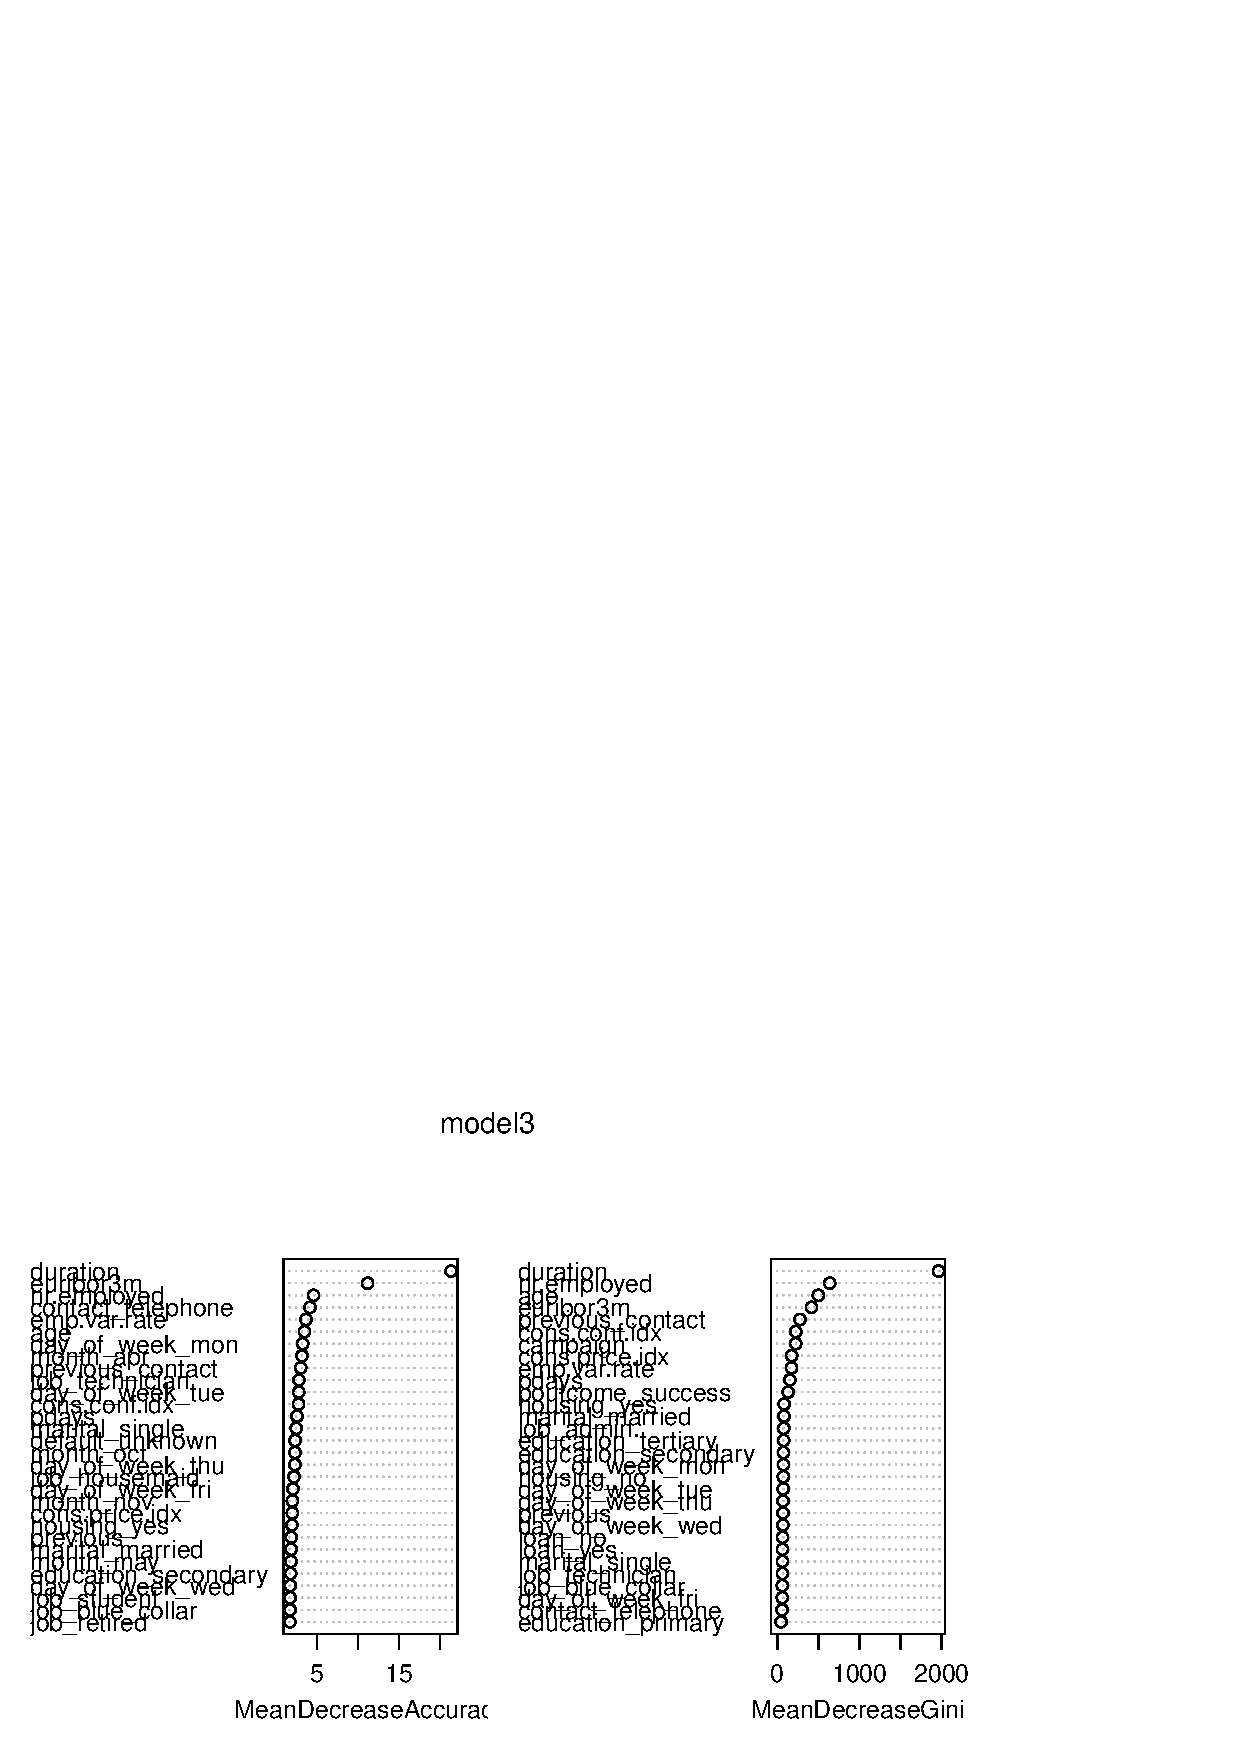
\includegraphics{apa10_files/figure-latex/unnamed-chunk-17-1.pdf}

\includegraphics{apa10_files/figure-latex/unnamed-chunk-18-1.pdf}

\includegraphics{apa10_files/figure-latex/unnamed-chunk-19-1.pdf}

\includegraphics{apa10_files/figure-latex/unnamed-chunk-20-1.pdf}

\includegraphics{apa10_files/figure-latex/unnamed-chunk-21-1.pdf}

\includegraphics{apa10_files/figure-latex/unnamed-chunk-22-1.pdf}

\includegraphics{apa10_files/figure-latex/unnamed-chunk-23-1.pdf}

\includegraphics{apa10_files/figure-latex/unnamed-chunk-24-1.pdf}

\includegraphics{apa10_files/figure-latex/unnamed-chunk-25-1.pdf}

\includegraphics{apa10_files/figure-latex/unnamed-chunk-26-1.pdf}

\includegraphics{apa10_files/figure-latex/unnamed-chunk-27-1.pdf}

\includegraphics{apa10_files/figure-latex/unnamed-chunk-28-1.pdf}

\includegraphics{apa10_files/figure-latex/unnamed-chunk-29-1.pdf}

\includegraphics{apa10_files/figure-latex/unnamed-chunk-30-1.pdf}

\includegraphics{apa10_files/figure-latex/unnamed-chunk-31-1.pdf}

\includegraphics{apa10_files/figure-latex/unnamed-chunk-32-1.pdf}

\includegraphics{apa10_files/figure-latex/unnamed-chunk-33-1.pdf}

\includegraphics{apa10_files/figure-latex/unnamed-chunk-34-1.pdf}

\includegraphics{apa10_files/figure-latex/unnamed-chunk-35-1.pdf}

\includegraphics{apa10_files/figure-latex/unnamed-chunk-36-1.pdf}

\subsubsection{Unique Value \& Missing
value}\label{unique-value-missing-value}

We see that there are no missing values in our dataset as shown in table
2 and graph format. The unique values are given in the table

\begin{longtable}[c]{@{}lr@{}}
\caption{Missing Values}\tabularnewline
\toprule
& Missing Values\tabularnewline
\midrule
\endfirsthead
\toprule
& Missing Values\tabularnewline
\midrule
\endhead
age & 0\tabularnewline
job & 0\tabularnewline
marital & 0\tabularnewline
education & 0\tabularnewline
default & 0\tabularnewline
housing & 0\tabularnewline
loan & 0\tabularnewline
contact & 0\tabularnewline
month & 0\tabularnewline
day\_of\_week & 0\tabularnewline
duration & 0\tabularnewline
campaign & 0\tabularnewline
pdays & 0\tabularnewline
previous & 0\tabularnewline
poutcome & 0\tabularnewline
emp.var.rate & 0\tabularnewline
cons.price.idx & 0\tabularnewline
cons.conf.idx & 0\tabularnewline
euribor3m & 0\tabularnewline
nr.employed & 0\tabularnewline
y & 0\tabularnewline
\bottomrule
\end{longtable}

\begin{longtable}[c]{@{}lr@{}}
\caption{Unique Values}\tabularnewline
\toprule
& Unique Values\tabularnewline
\midrule
\endfirsthead
\toprule
& Unique Values\tabularnewline
\midrule
\endhead
age & 78\tabularnewline
job & 12\tabularnewline
marital & 4\tabularnewline
education & 8\tabularnewline
default & 3\tabularnewline
housing & 3\tabularnewline
loan & 3\tabularnewline
contact & 2\tabularnewline
month & 10\tabularnewline
day\_of\_week & 5\tabularnewline
duration & 1544\tabularnewline
campaign & 42\tabularnewline
pdays & 27\tabularnewline
previous & 8\tabularnewline
poutcome & 3\tabularnewline
emp.var.rate & 10\tabularnewline
cons.price.idx & 26\tabularnewline
cons.conf.idx & 26\tabularnewline
euribor3m & 316\tabularnewline
nr.employed & 11\tabularnewline
y & 2\tabularnewline
\bottomrule
\end{longtable}

\subsubsection{Data Summary post
conversion}\label{data-summary-post-conversion}

\subsubsection{Outliers Analysis}\label{outliers-analysis}

\includegraphics{apa10_files/figure-latex/unnamed-chunk-39-1.pdf}

\subsubsection{Analysis of link functions for given
variables}\label{analysis-of-link-functions-for-given-variables}

\subsection{R Code}\label{r-code}

\setlength{\parindent}{-0.5in} \setlength{\leftskip}{0.5in}
\setlength{\parskip}{11pt}



\end{document}
